\chapter{绪论}

\section{研究背景}

以下为一段文字

视频提供了功能强大的方法帮助您证明您的观点。当您单击联机视频时,可以在想要添加的视频的嵌入代码中进行粘贴。您也可以键入一个关键字以联机搜索最适合您的文档的视频。
为使您的文档具有专业外观,提供了页眉、页脚、封面和文本框设计,这些设计可互为补充。例如,您可以添加匹配的封面、页眉和提要栏。单击“插入”,然后从不同库中选择所需元素。
主题和样式也有助于文档保持协调。当您单击设计并选择新的主题时,图片、图表或 SmartArt 图形将会更改以匹配新的主题。当应用样式时,您的标题会进行更改以匹配新的主题。
\par 使用在需要位置出现的新按钮在 Word 中保存时间。若要更改图片适应文档的方式,请单击该图片,图片旁边将会显示布局选项按钮。当处理表格时,单击要添加行或列的位置,然后单击加号。
在新的阅读视图中阅读更加容易。可以折叠文档某些部分并关注所需文本。如果在达到结尾处之前需要停止读取,Word 会记住您的停止位置 - 即使在另一个设备上
。
\subsection{技术应用}
当双耳渲染技术足够成熟时,其应用包括:
\begin{itemize}[leftmargin=*]
\item 提高语言通信的可懂度。目前绝大部分的语言通信采用的是单通路的信号传输系统,不能实现目标语言声源与其他声源在空间上分离,因而语言可懂度会变差。如果引入双耳渲染技术,对原始场景进行重现保留声源的空间信息,就可以提高语言通信的质量;
\item 引导视觉定位。声音信息的空间化可以引导视觉定位,甚至可以在不借助视觉的情况下寻找目标,从而减少寻找目标以及采取应对措施的时间,提高安全性。主要用途是民用或军用救援搜索、旅游或博物馆向导、盲人的导向和信息系统;\cite{liu_approaching_2018},如图\ref{picexam}所示。
\item 提高语言通信的可懂度。目前绝大部分的语言通信采用的是单通路的信号传输系统,不能实现目标语言声源与其他声源在空间上分离,因而语言可懂度会变差。如果引入双耳渲染技术,对原始场景进行重现保留声源的空间信息,就可以提高语言通信的质量;
\item 引导视觉定位。声音信息的空间化可以引导视觉定位,甚至可以在不借助视觉的情况下寻找目标,从而减少寻找目标以及采取应对措施的时间,提高安全性。主要用途是民用或军用救援搜索、旅游或博物馆向导、盲人的导向和信息系统;\cite{liu_approaching_2018},如图\ref{picexam}所示。
\item 提高语言通信的可懂度。目前绝大部分的语言通信采用的是单通路的信号传输系统,不能实现目标语言声源与其他声源在空间上分离,因而语言可懂度会变差。如果引入双耳渲染技术,对原始场景进行重现保留声源的空间信息,就可以提高语言通信的质量;
\item 引导视觉定位。声音信息的空间化可以引导视觉定位,甚至可以在不借助视觉的情况下寻找目标,从而减少寻找目标以及采取应对措施的时间,提高安全性。主要用途是民用或军用救援搜索、旅游或博物馆向导、盲人的导向和信息系统;\cite{liu_approaching_2018},如图\ref{picexam}所示。
\end{itemize}

\section{图片}
视频提供了功能强大的方法帮助您证明您的观点。当您单击联机视频时,可以在想要添加的视频的嵌入代码中进行粘贴。您也可以键入一个关键字以联机搜索最适合您的文档的视频。
为使您的文档具有专业外观,Word 提供了页眉、页脚、封面和文本框设计,这些设计可互为补充。例如,您可以添加匹配的封面、页眉和提要栏。单击“插入”,然后从不同库中选择所需元素。
主题和样式也有助于文档保持协调。当您单击设计并选择新的主题时,图片、图表或 SmartArt 图形将会更改以匹配新的主题。当应用样式时,您的标题会进行更改以匹配新的主题。
使用在需要位置出现的新按钮在 Word 中保存时间。若要更改图片适应文档的方式,请单击该图片,图片旁边将会显示布局选项按钮。当处理表格时,单击要添加行或列的位置,然后单击加号。
在新的阅读视图中阅读更加容易。可以折叠文档某些部分并关注所需文本。如果在达到结尾处之前需要停止读取,Word 会记住您的停止位置 - 即使在另一个设备上
\begin{figure}[H]
	\centering
	
\includegraphics[width=0.6\textwidth]{figure/chapter1/Omni.jpg}
	\bicaption{不带子图图片示例,(a)1,(b)2,(c)3,(d)4}{This is an english title}
	\label{picexam}
\end{figure}
视频提供了功能强大的方法帮助您证明您的观点。当您单击联机视频时,可以在想要添加的视频的嵌入代码中进行粘贴。您也可以键入一个关键字以联机搜索最适合您的文档的视频。
为使您的文档具有专业外观,Word 提供了页眉、页脚、封面和文本框设计,这些设计可互为补充。例如,您可以添加匹配的封面、页眉和提要栏。单击“插入”,然后从不同库中选择所需元素。
主题和样式也有助于文档保持协调。当您单击设计并选择新的主题时,图片、图表或 SmartArt 图形将会更改以匹配新的主题。当应用样式时,您的标题会进行更改以匹配新的主题。
\begin{figure}[H]
	\centering
	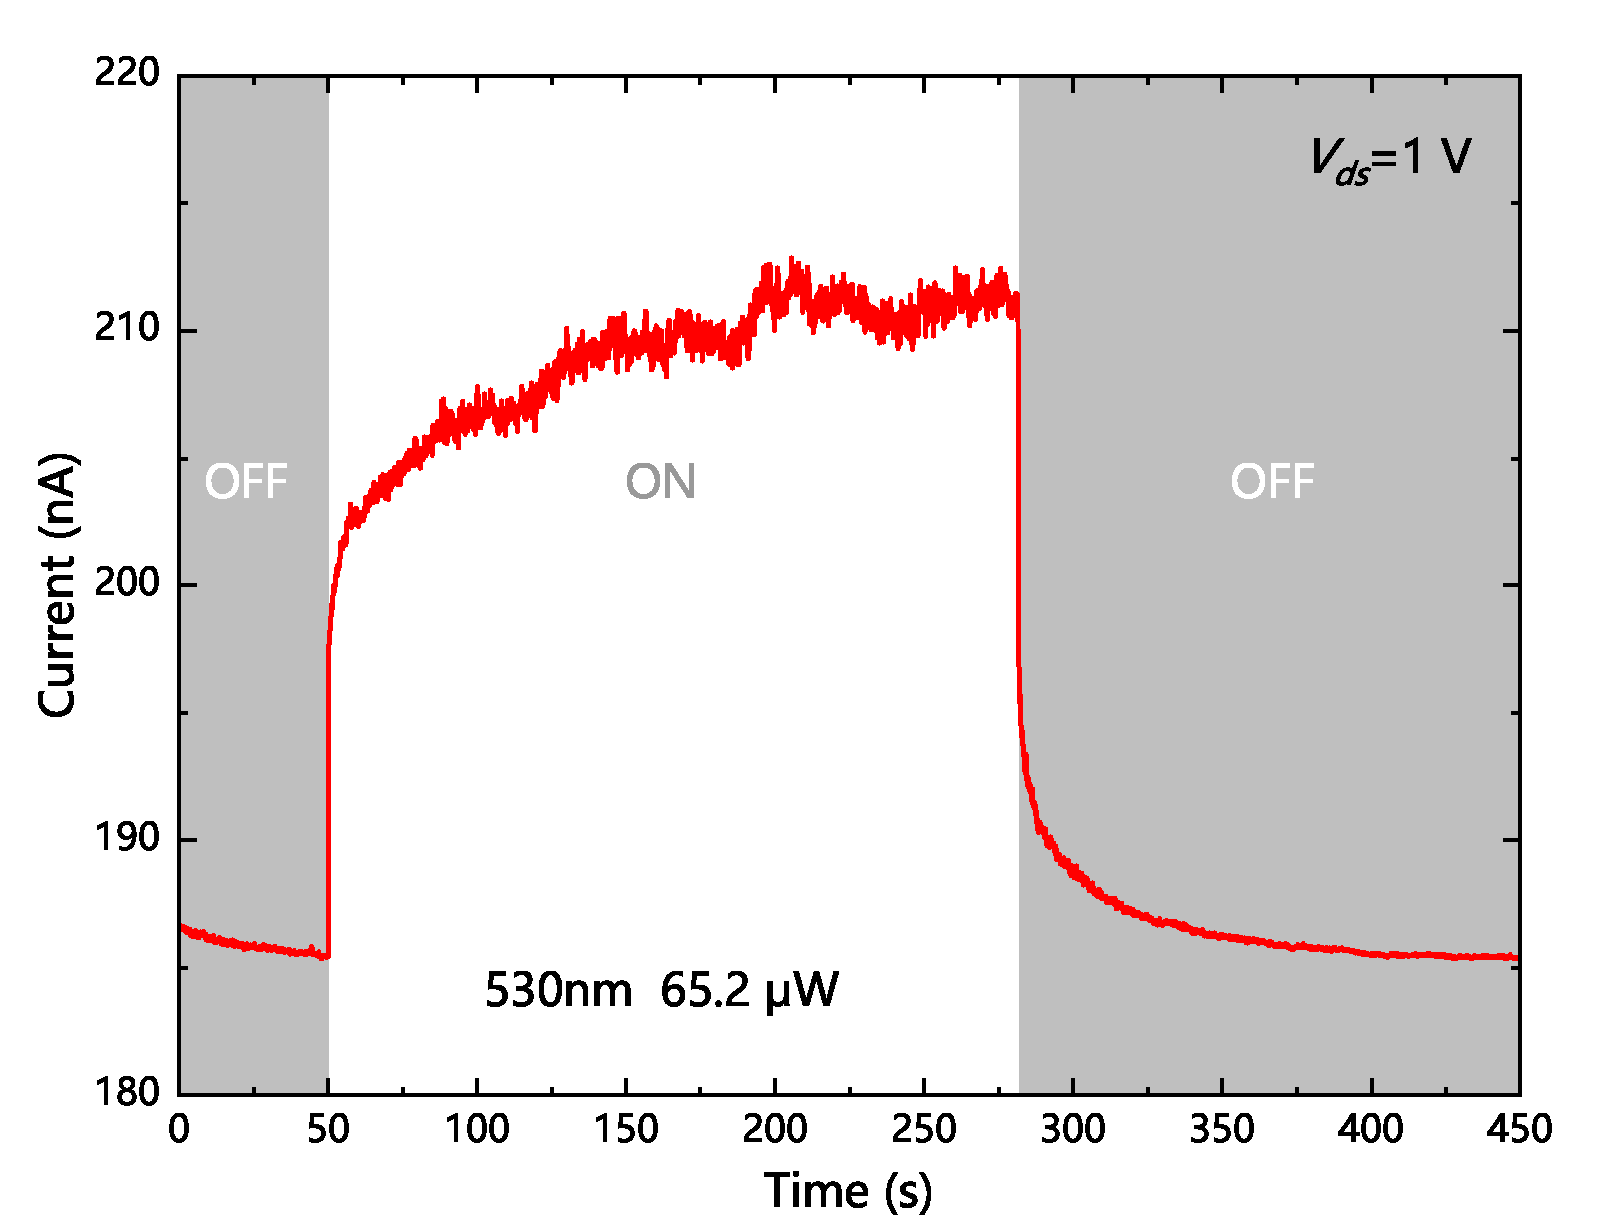
\includegraphics[width=0.6\textwidth]{figure/chapter1/Graph3.pdf}
	\caption{矢量图片示例,无英文标题}	
	\label{pdfpic}
\end{figure}
使用在需要位置出现的新按钮在 Word 中保存时间。若要更改图片适应文档的方式,请单击该图片,图片旁边将会显示布局选项按钮。当处理表格时,单击要添加行或列的位置,然后单击加号。
在新的阅读视图中阅读更加容易。可以折叠文档某些部分并关注所需文本。如果在达到结尾处之前需要停止读取,Word 会记住您的停止位置 - 即使在另一个设备上

如果要引用图片,实例:图\ref{pdfpic}所示,注意图片要加 label且不可重复

\textcolor{red}{添加了对双语标题的支持},图片其实不太推荐\LaTeX 子图,建议拼好放进来

\begin{figure}[H]
\centering
\subfigure[]{

\includegraphics[width=0.21\textwidth]{figure/chapter1/Omni.jpg}}
\subfigure[]{

\includegraphics[width=0.21\textwidth]{figure/chapter1/Omni.jpg}}\\
\subfigure[]{

\includegraphics[width=0.21\textwidth]{figure/chapter1/Omni.jpg}}
\hspace{3cm}
\subfigure[]{

\includegraphics[width=0.21\textwidth]{figure/chapter1/Omni.jpg}}

\bicaption{带子图图片示例,(a)1,(b)2,(c)3,(d)4}{This is an english figure title}
\label{fig:binaural_recording}
\end{figure}

视频提供了功能强大的方法帮助您证明您的观点。当您单击联机视频时,可以在想要添加的视频的嵌入代码中进行粘贴。您也可以键入一个关键字以联机搜索最适合您的文档的视频。
为使您的文档具有专业外观,Word 提供了页眉、页脚、封面和文本框设计,这些设计可互为补充。例如,您可以添加匹配的封面、页眉和提要栏。单击“插入”,然后从不同库中选择所需元素。
主题和样式也有助于文档保持协调。当您单击设计并选择新的主题时,图片、图表或 SmartArt 图形将会更改以匹配新的主题。当应用样式时,您的标题会进行更改以匹配新的主题。

\section{表格}
\begin{tabular}{ccc}
	&  &  \\
	&  &  \\
\end{tabular}
\begin{table}[H]
\caption{HRTF 预处理方法}
\centering
\begin{tabular}{|c|c|c|}
\hline
方法 & 预处理对象 & 预处理方法 \\
\hline
$H_{a}$ & 复频谱 & 时间对准 \\
$H_{s m}$ & \multicolumn{1}{l|}{复频谱} & 平滑 \\
$|H|$ & 幅度谱 & 无 \\

\hline
\end{tabular}
\end{table}
视频提供了功能强大的方法帮助您证明您的观点。当您单击联机视频时,可以在想要添加的视频的嵌入代码中进行粘贴。您也可以键入一个关键字以联机搜索最适合您的文档的视频。
为使您的文档具有专业外观,Word 提供了页眉、页脚、封面和文本框设计,这些设计可互为补充。例如,您可以添加匹配的封面、页眉和提要栏。单击“插入”,然后从不同库中选择所需元素。
主题和样式也有助于文档保持协调。当您单击设计并选择新的主题时,图片、图表或 SmartArt 图形将会更改以匹配新的主题。当应用样式时,您的标题会进行更改以匹配新的主题。
\subsection{三线表}
\begin{table}[H]
	\caption{HRTF 预处理方法}
	\centering
	\begin{tabular*}{\hsize}{@{\extracolsep{\fill}}ccc}
		\toprule
		方法 & 预处理对象 & 预处理方法 \\
		\midrule
		$H_{a}$ & 复频谱 & 时间对准 \\
		$H_{s m}$ & 复频谱 & 平滑 \\
		$|H|$ & 幅度谱 & 无 \\
		\bottomrule
	\end{tabular*}
	\label{tab.pre_processing}
\end{table}
视频提供了功能强大的方法帮助您证明您的观点。当您单击联机视频时,可以在想要添加的视频的嵌入代码中进行粘贴。您也可以键入一个关键字以联机搜索最适合您的文档的视频。
为使您的文档具有专业外观,Word 提供了页眉、页脚、封面和文本框设计,这些设计可互为补充。例如,您可以添加匹配的封面、页眉和提要栏。单击“插入”,然后从不同库中选择所需元素。
主题和样式也有助于文档保持协调。当您单击设计并选择新的主题时,图片、图表或 SmartArt 图形将会更改以匹配新的主题。当应用样式时,您的标题会进行更改以匹配新的主题。
\begin{table}[htbp]
	\centering
	\bicaption{主要仪器设备}{Main devices used}
	\label{instruments}
	\renewcommand\arraystretch{1.5}
	\zihao{5}
	\begin{tabular*}{\hsize}{@{}@{\extracolsep{\fill}}ccc@{}}
		\toprule
		仪器名称          &      型号       &      生产厂家      \\ 
		\midrule
		超纯水系统         &   CSR-1-10    & 北京爱斯泰克科技开发有限公司 \\
		电热恒温鼓风干燥箱     &   DGG-9030B   &  上海森信实验仪器有限公司  \\
		分析天平          &    AUW220D    &    日本岛津制作所     \\
		程序升温箱式炉       &   KSL 1200X   &   合肥科晶材料有限公司   \\
		恒温加热磁力搅拌器     &     CL-4      &  巩义市予华仪器有限公司   \\
		程序升温管式炉       &    KSL YDL    &   扬州宝鼎电热电器厂    \\
		X射线衍射分析仪      &  X’pert pro   &    日本Rigaku    \\
		场发射扫描电子显微镜    &   JSM-7001F   & 日本电子株式会社(JEOL) \\
		紫外可见分光光度计     &   UV-9000S    &   上海元析仪器有限公司   \\
		%		  & 	Escalab 250Xi & 赛默飞世尔科技公司\\
		离心机          &    TDL-6A     & 上海菲恰尔分析仪器有限公司  \\
		\bottomrule
	\end{tabular*}
\end{table}
视频提供了功能强大的方法帮助您证明您的观点。当您单击联机视频时,可以在想要添加的视频的嵌入代码中进行粘贴。您也可以键入一个关键字以联机搜索最适合您的文档的视频。
为使您的文档具有专业外观,Word 提供了页眉、页脚、封面和文本框设计,这些设计可互为补充。例如,您可以添加匹配的封面、页眉和提要栏。单击“插入”,然后从不同库中选择所需元素。
主题和样式也有助于文档保持协调。当您单击设计并选择新的主题时,图片、图表或 SmartArt 图形将会更改以匹配新的主题。当应用样式时,您的标题会进行更改以匹配新的主题。视频提供了功能强大的方法帮助您证明您的观点。当您单击联机视频时,可以在想要添加的视频的嵌入代码中进行粘贴。您也可以键入一个关键字以联机搜索最适合您的文档的视频。
为使您的文档具有专业外观,Word 提供了页眉、页脚、封面和文本框设计,这些设计可互为补充。例如,您可以添加匹配的封面、页眉和提要栏。单击“插入”,然后从不同库中选择所需元素。
主题和样式也有助于文档保持协调。当您单击设计并选择新的主题时,图片、图表或 SmartArt 图形将会更改以匹配新的主题。当应用样式时,您的标题会进行更改以匹配新的主题。视频提供了功能
为使您的文档具有专业外观,Word 提供了页眉、页脚、封面和文本框设计,这些设计可互为补充。例如,您可以添加匹配的封面、页眉和提要栏。单击“插入”,然后从不同库中选择所需元素。
主题和样式也有助于文档保持协调。当您单击设计并选择新的主题时,图片、图表或 SmartArt 图形将会更改以匹配新的主题。当应用样式时,您的标题会进行更改以匹配新的主题。

\begin{table*}
	\centering
	\caption{Comparison of different obfuscations in terms of their transformation capabilities}
	\begin{tabular}{ccccc} % 控制表格的格式
		\toprule
		\multirow{2}{*}{Obfuscators} & \multicolumn{4}{c}{Transformations}   \\
		\cline{2-5}  % 这部分是画一条横线在2-6 排之间
		&    Renaming & Dead code removal & control flow obfuscation & string encryption \\
		\midrule
		Proguard &  \checkmark & $\times$  & $\times$ & \checkmark   \\
		Allatori & \checkmark & $\times$  & $\times$ & \checkmark \\
		DashO & \checkmark & $\times$  & $\times$ & \checkmark \\
		Androcrypt & \checkmark & $\times$  & $\times$ & \checkmark  \\
		\bottomrule
	\end{tabular}
	\label{tbl:table1}
\end{table*}

\section{公式}
从~SOFA~格式角度定义到最终角度定义的转换公式为:
\[
M=
\left[
\begin{matrix}
	\textcolor{red}{\varepsilon_{11}} & \varepsilon_{12} & \varepsilon_{13}\\
	\varepsilon_{21} & \varepsilon_{22} & \varepsilon_{23}\\
	\varepsilon_{31} & \varepsilon_{32} & \varepsilon_{33}\\
\end{matrix}\right]
\]

\begin{align}
	\label{111}
	\phi & = \text{mod}~\left( 360^{\circ}-\varphi_{\text{SOFA}}, 360^{\circ} \right)  \nonumber \\
	\theta & =  90^{\circ} - \theta_{\text{SOFA}} 	
\end{align}

\[
\mu = \frac{B}{H}=\frac{B_0 e^{i\omega t-\delta}}{H_0 e^{i\omega t}}=\frac{B_0}{H_0}\cos\delta-i\frac{B_0}{H_0}\sin\delta
\]
其中,mod~表示取余。详见 式\ref{111}
\begin{equation}
\eta = \frac{qVN_0}{d^2}\left\{(\mu\tau)_e \left[1-\text{exp}\left(\frac{x_0-d}{\frac{(\mu\tau)_e V}{d}}\right)\right]+(\mu\tau)_h \left[1-\text{exp}\left(\frac{-x_0}{\frac{(\mu\tau)_h V}{d}}\right)\right]\right\}
\end{equation}
